\chapter{Conceptos previos}
\section{Definición electrónica digital}
La electrónica digital es el campo en donde se estudian circuitos electrónicos que funcionan con lógica digital. Estos se basan en señales digitales que se interpretan en base a dos valores lógicos: 0 y 1. Estas son distintas a las señales analógicas, ya que usan rangos de valores, también se usa para manipulación de dígitos binarios con la función de administrar procesos y la implementación de sistemas electrónicos en los cuales la información esta codificada en dos estados, entregándole la capacidad de procesar y controlar varios sistemas y subsistemas.


\begin{figure}[hbt!]
  \centering
  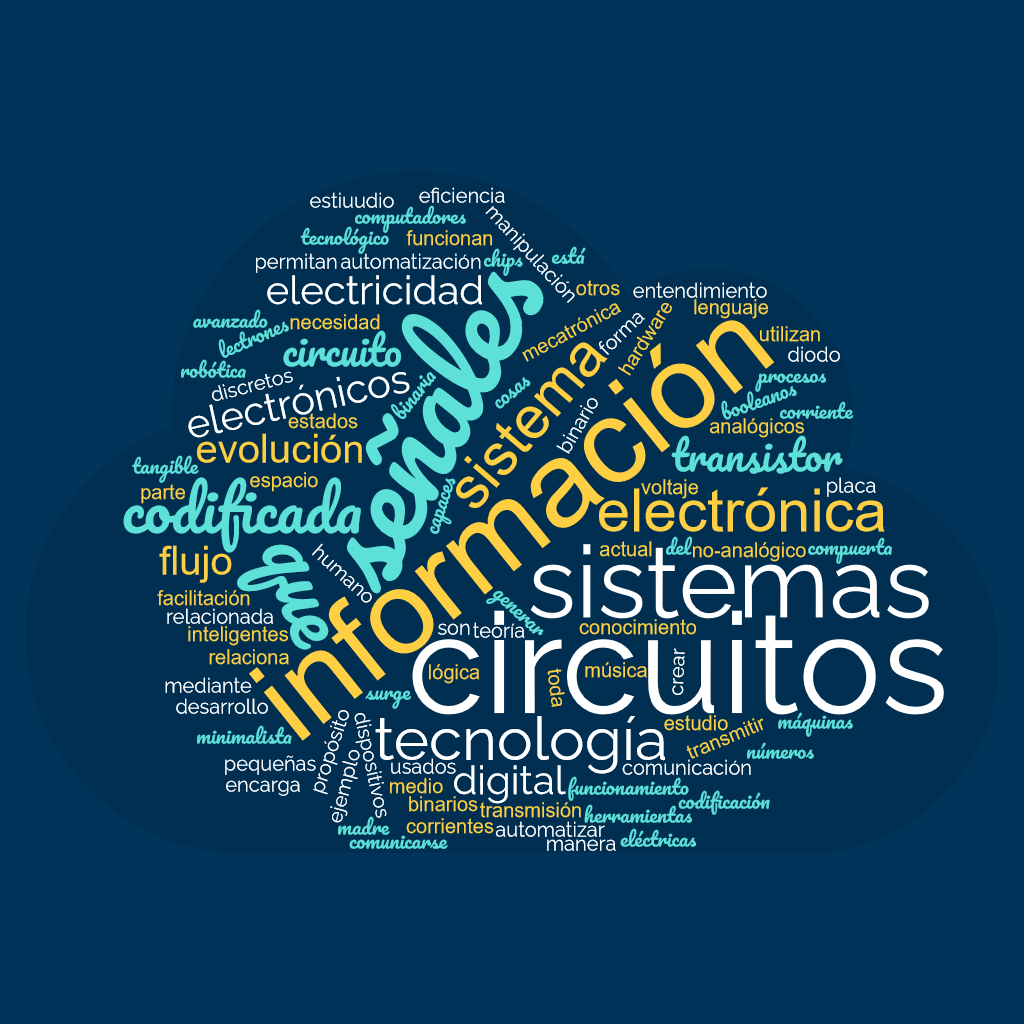
\includegraphics[width=\textwidth]{electronicadigital.png}
  \caption{Nube de palabras en base a los conceptos señalados para el término "Electrónica Digital"}
\end{figure}

\section{Componentes de los circuitos eléctricos} %Jose Acosta

\begin{itemize}
    \item Resistencia/Resistor:

Un resistor o resistencia es un componente electrónico que se opone al flujo de la corriente por este. Tienen dos terminales (entrada y salida) que no poseen polaridad, por lo tanto, no importa la orientación al momento de conectarlo.

\item Fuente de Voltaje:

Componente eléctrico que genera una diferencia de potencial (voltaje) de salida.

\item Fuente de corriente: Es un componente que proporciona corriente eléctrica al circuito.

\item Switch/interruptor:  dispositivo que permite abrir, cerrar o desviar un circuito eléctrico.
\end{itemize}

\section{Variables eléctricas}
Para el análisis de circuitos eléctricos  se debe conocer ciertos conceptos básicos que están directamente relacionado, Los cuales son:
\begin{itemize}
    \item Corriente Eléctrica: es un fenómeno físico causado por el desplazamiento de una carga, pudiendo ser flujo de electrones o de iones.
    
    \item Tensión Eléctrica: o diferencia de potencial es una magnitud física que indica la diferencia de potencial entre 2 de un circuito eléctrico.
    
    \item Potencia Eléctrica: Es la proporción de corriente eléctrica que transfiere un circuito eléctrico por unidad de tiempo, es decir, energía disipada durante un periodo de tiempo. se expresa en Watt[W]. Otra forma de representarlo es la cantidad de energía eléctrica transferida de una fuente de alimentación o generadora a un elemento consumido por unidad de tiempo
    
\end{itemize}

\section{Simbología circuitos} %Valeska Acuña

Hay una gran cantidad de componentes empleados en los diseños de circuitos, a continuación se presentarán la simbología de los elementos más comunes utilizados para esquematizar circuitos eléctricos.
Cabe destacar que elementos como las fuentes de corriente, fuentes de voltajes, resistencias, entre otros, tienen distintas representaciones, por lo que hay que considerar las existencias de estas para evitar confusiones.\\


\begin{circuitikz}

\draw (0,0) to[american voltage source, l=Fuente de Voltaje] ++(3,0)
(5,0) to[american controlled voltage source, l= Fuente de Voltaje Dependiente] ++(3,0) 
(10,0) to[american current source, l= Fuente de Corriente] ++(3,0);\\
\draw (0,-2) to[american controlled current source, l= Fuente de Corriente Dependiente] ++(3,0) 
(5,-2) to[battery, l = Batería] ++(3,0) 
(10,-2) to[battery1,l=Batería] ++(3,0);\\
\draw (0,-4) to[sinusoidal voltage source, l = Fuente Sinusoidal] ++(3,0) 
(5,-4) to[R,l=Resistencia] ++(3,0) 
(10,-4) to[european resistor, l= Resistencia] ++(3,0);\\
\draw (0,-6) to[capacitor, l=Capacitor] ++(3,0) 
(5,-6) to[inductor, l= Inductor] ++(3,0)
(10,-6) to[normal open switch, l= Switch] ++(3,0);\\
\draw (0,-8) to[empty diode, l=Diodo] ++(3,0) (5,-8) to[ammeter, l= Amperímetro] ++(3,0) (10,-8) to[voltmeter, l= Voltímetro] ++(3,0);\\
\draw (0,-10) to[empty led, l=LED] ++(3,0) %\node[ground, label=above:Tierra, scale = 2]() at (6.5,-9.5)  ++(3,0) 
%
%\node[npn, label=right:Transistor](npn) (11.5,-10) 
;
\end{circuitikz}

%Fin Valeska Acuña
Por otro lado, consideraremos que los cables cruzados no están conectados a menos que sea un cruce en T o con un punto:
 

\begin{circuitikz}

\draw (0,0) to ++(3,0) (3,0) to ++(0,3)
(4,0) to ++(3,0) (5.5,0) to ++(0,3) 
(8,1.5) to ++(3,0) (9.5,0) to ++(0,3) 
(12,1.5) to ++(3,0) (13.5,0)   to[short,-*]++(0,1.5) to ++(0,1.5) ;
\end{circuitikz}

\section{Definición cortocircuito, circuito abierto y cerrado}
%Inicio Javiera Alvarez
\begin{itemize}
    \item Circuito Cerrado: Un circuito se denomina cerrado cuando existe un camino cerrado, continuo; permitiendo que fluya la corriente eléctrica.
    \newline
    \item Cortocircuito:  circuito cerrado con una conexión directa entre dos terminales de un componente eléctrico. La corriente eléctrica toma el camino de menor resistencia, por lo que en un cortocircuito la corriente pasará por alto los caminos paralelos y viajará a través de la conexión directa.Esto provoca una corriente infinita, lo que probablemente derrita el aislamiento del cable y podría provocar un incendio u otros problemas asociados
    \newline
    \item Circuito abierto: corresponde a un circuito en que no fluye corriente ya que hay una discontinuidad de su camino. Cualquier circuito que no tenga un camino de retorno es un circuito abierto.
\end{itemize}

%\begin{figure}[hbt!]
%  \centering
%  \includegraphics[scale=0.3]{figure/circuitos.png}
%\end{figure}

\begin{figure}

             \centering
     
     
     \begin{subfigure}{0.3\textwidth}
             \centering
             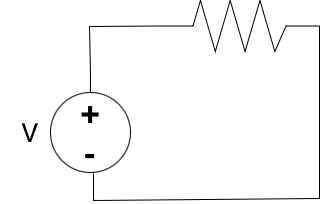
\includegraphics
[width=\textwidth]{images/C01/CircuitoCerrado.png}
         \caption{Circuito Cerrado}
         \label{fig:circCerrado}
     \end{subfigure}

     \begin{subfigure}{0.3\textwidth}
             \centering
             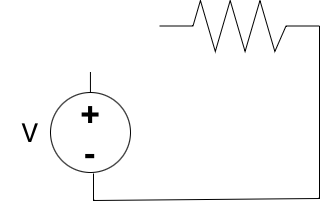
\includegraphics[width=\textwidth]{images/C01/C01-CircuitoAbierto.png}
         \caption{Circuito Abierto}
         \label{fig:circAbierto}
     \end{subfigure}
     

     \begin{subfigure}{0.3\textwidth}
             \centering
             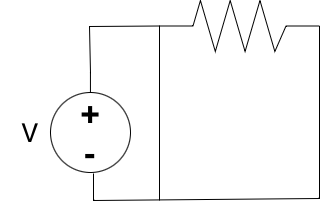
\includegraphics[width=\textwidth]{images/C01/CortoCircuito.png}
         \caption{Corto Circuito}
         \label{fig:CortoCirc}
     \end{subfigure}
     
     
     
     
     
        \caption{Ejemplos de condiciones de circuito}
        \label{fig:ejemplosCondiciones}
\end{figure}

    
    
    
    
        
%Fin Javiera Alvarez


